\documentclass{scrartcl}
\usepackage[T1]{fontenc}
\usepackage[utf8]{inputenc}
\usepackage[ngerman]{babel}
\usepackage{amsmath,amssymb}
\usepackage{graphicx}
\usepackage{enumerate}

\usepackage{tikz}
\usepackage{tabto}

\definecolor{darkred}{rgb}{0.53,0,.08}

\tikzstyle{rvertex}=[circle,fill=white,minimum size=23pt, inner sep=0pt, text=black, line width=1pt, draw=darkred, font=\Large]
\tikzstyle{bvertex}=[circle,fill=black,minimum size=23pt, inner sep=0pt, text=white, line width=1pt, draw=black, font=\Large]
\tikzstyle{nilvertex}=[rectangle,fill=black,minimum size=12pt, inner sep=0pt, text=white, line width=1pt, draw=black, text width=0.2cm, font=\scriptsize, align=center]
\tikzstyle{niceedge}=[draw, very thick, ->, gray]
\newcommand{\nil}{N\newline I\newline L}

\newcommand{\rbt}{Rot-Schwarz-Baum }


\begin{document}
\TabPositions{0.8cm, 1.6cm, 2.4cm, 3.2cm}

\begin{center}
	{\huge \textbf{Algorithmen I} \\
			\textbf{Übungsklausur}\\
			\textbf{Musterlösung} \\
			\textbf{11.07.2012}}
\end{center}
\textbf{Name:}\\
\section*{Aufgabe 1: Wissensfragen (6 Punkte)}
\begin{enumerate}[(1)]
\item Nennen Sie zwei in der Vorlesung vorgestellte Algorithmen, die nach dem Greedy-Prinzip arbeiten. Begründen Sie kurz, warum. (1P)\\
\textbf{mögliche Lösungen:}
\begin{itemize}
\item Kruskal: es wird immer die Kante mit dem niedrigsten Gewicht ausgewählt, die Teil eines minimalen Spannbaums sein kann.
\item Prim: es wird immer die leichteste Kante, die den bisherigen MST mit einem neuen Knoten verbindet, ausgewählt.
\item Dijkstra: Durch die Verwendung einer Prioritätswarteschlange werden immer die ausgehenden Kanten des Knotens mit der geringsten Distanz relaxiert.
\end{itemize}

\item Nennen Sie einen Vorteil und einen Nachteil von Mergesort gegenüber Quicksort. (1P)\\
\textbf{mögliche Lösungen:}
\begin{itemize}
\item[(+)] besseres Verhalten im Worst Case
\item[(+)] stabil
\item[(-)] im Durchschnitt eher langsamer als Quicksort
\item[(-)] zusätzlicher Speicher benötigt (nicht in-place)
\end{itemize}

\item Was bedeutet Stabilität bei Sortieralgorithmen? Nennen Sie eine Situation, in der man die Stabilität ausnutzen kann. (2P)\\
\textbf{Lösung:}\\
Stabilität bedeutet, dass sich die Reihenfolge von gleichen Elementen beim Sortieren nicht ändern. Anwenden lässt sich diese z.B. bei Tupeln, die lexikographisch geordnet werden (d.h. zuerst nach dem ersten Wert, bei Gleichheit nach dem zweiten). Ein Beispiel hierfür wären Tupel der Form (Monat, Tag) für einen Tag innerhalb eines Jahres. Man sortiert dabei zuerst nach dem zweiten Wert und danach mit einem stabilen Sortieralgorithmus nach dem ersten Wert. Bei Tupeln mit gleicher erster Komponente wird dann nämlich die ursprüngliche Reihenfolge beibehalten, welche durch Sortieren nach der zweiten Komponente erreicht wurde.

\item Zeigen oder widerlegen Sie: Bin\"are Suche hat auf jeder Datenstruktur eine bessere Laufzeit als Lineare Suche. (2P)\\
\textbf{Lösung:}\\
Die Behauptung ist falsch! Beispielsweise bringt binäre Suche keinen Geschwindigkeitsvorteil bei einer verketteten Liste, da sie keinen wahlfreien Zugriff in O(1) erlaubt.
\end{enumerate}

\section*{Aufgabe 2: Heaps (12 Punkte)}
\begin{enumerate}[(1)]
\item Gegeben sei das folgende Feld: \\
\ \\
\begin{tabular}{|c|c|c|c|c|c|c|c|c|c|c|}
\hline
12 & 21 & 19 & 26 & 99 & 30 & 24 & 32 & 18 & 101 & 128 \\ 
\hline 
\end{tabular} \\
\begin{enumerate}[(a)]
	\item Erläutern Sie, warum das Feld keinen gültigen Min-Heap darstellt. (1P)\\
	\textbf{Lösung}:\\
	Das Element mit dem Schlüssel 18 verletzt die Heap-Eigenschaft, da es kleiner als 26 und 21 ist, aber weiter unten als diese im Heap steht.
	
	\item Reparieren Sie den Min-Heap mit dem aus der Vorlesung bekannten Verfahren. Geben Sie dabei den Heap nach jeder Änderung an (als Feld oder als Baum). (3P)\\
\textbf{Lösung:}\\
\begin{verbatim}
          12                              12 
       /       \                       /       \
     21         19                   21          19
   /   \       /   \       ->      /   \        /   \
  26    99    30   24             18     99    30   24
 / \   /  \                       / \   /  \
32 18 101 128                    32 26 101 128

             12 
         /       \
       18         19
->   /   \       /   \
    21    99    30   24
   / \   /  \
  32 26 101 128
\end{verbatim}
\end{enumerate}

\item \begin{enumerate}[(a)]
	\item Warum l\"asst sich in einem Heap, egal wie gut er implementiert ist, das Minimum nicht in $\Theta(1)$ entfernen, sodass die entstehende Struktur immer noch ein Heap ist? (4P) \newline
Hinweis: Betrachten Sie die Laufzeit einer Heapsort-Implementierung, wenn dies möglich wäre. Welcher Widerspruch ergibt sich daraus?\\
\textbf{Lösung:}\\
Der Heap l\"asst sich in $\Theta(n)$ aufbauen. Wenn das Extrahieren des Minimums jedes Mal $\Theta(1)$ braucht, dauern alle Extrahierungsaktionen zusammen $\Theta(n)$, da man diesen Schritt während des Sortiervorgangs $n$ Mal macht. Es ergibt sich eine Gesamtlaufzeit von $\Theta(n)$, was der unteren Schranke des Sortierproblems ($\Theta(nlog(n)$) widerspricht.

	\item Geben Sie eine Datenstruktur an, die die entsprechende Eigenschaft aus (a) hat. (3P)\\
	\textbf{Lösung:}\\
	Eine aufsteigend sortierte verkettete Liste erf\"ullt genau das gew\"unschte (Extrahieren des Minimums ist dann einfach "`remove head"').


	\item Warum ist dies kein Widerspruch zur \"Uberlegung aus (a)? (1P)\\
	\textbf{Lösung:}\\
	Beim Aufbau dieser Datenstruktur muss die Liste sortiert werden. Dies braucht wegen der unteren Schranke mindestens $\Theta(n\log n)$. F\"ur ein Sortierverfahren ist der Aufbau der Datenstruktur aber n\"otig. Also widerspricht dies nicht den \"Uberlegungen aus (a).

\end{enumerate}
\end{enumerate}


\section*{Aufgabe 3: Sortieren (13 Punkte)}
\begin{enumerate}[(1)]
\item Gegebenen sei der Sortieralgorithmus \emph{Cocktail-Sort}. Um ein Array zu sortieren, durchschreitet der Algorithmus das Array zun\"achst von vorne nach hinten und vertauscht dabei zwei benachbarte Werte, wenn sie in der falschen Reihenfolge stehen. Ist der Algorithmus am Ende des Arrays angekommen, durchschreitet er das Array jetzt in umgekehrter Reihenfolge von hinten nach vorne (bewegt sich also \glqq wieder zur\"uck\grqq). Dies wird so lange fortgesetzt, bis in einem Durchlauf keine Elemente mehr vertauscht werden.
\begin{enumerate}[(a)]
\item Wenden Sie Cocktail-Sort auf folgendes Array an, um die Elemente \textbf{aufsteigend} zu sortieren. Geben Sie dabei das Array nach jedem Schritt an. (3P)
\\
\begin{center}
\begin{tabular}{|c|c|c|c|c|c|}
\hline
4 & 2 & 1 & 3 & 7 & 3 \\
\hline
\end{tabular}
\end{center}
\text{ } \\
\textbf{Lösung:}\\
\begin{center}
\begin{tabular}{|c|c|c|c|c|c|}
\hline
4 & 2 & 1 & 3 & 7 & 3 \\
\hline
2 & 4 & 1 & 3 & 7 & 3 \\
\hline
2 & 1 & 4 & 3 & 7 & 3 \\
\hline
2 & 1 & 3 & 4 & 7 & 3 \\
\hline
2 & 1 & 3 & 4 & 7 & 3 \\
\hline
2 & 1 & 3 & 4 & 3 & 7 \\
\hline
2 & 1 & 3 & 4 & 3 & 7 \\
\hline
2 & 1 & 3 & 3 & 4 & 7 \\
\hline
2 & 1 & 3 & 3 & 4 & 7 \\
\hline
2 & 1 & 3 & 3 & 4 & 7 \\
\hline
1 & 2 & 3 & 3 & 4 & 7 \\
\hline
\end{tabular}
\end{center}

\item Geben Sie eine naive Implementierung von \emph{Cocktail-Sort} in Pseudocode an. (7P)\\
\textbf{Lösung:}\\
\textit{COCKTAIL-SORT(A)}\\
01 \tab \textbf{do} \\
02 \tab \tab vertauscht = \textbf{false};\\
03 \tab \tab \textbf{for} i = 1 \textbf{to} A.länge - 1\\
04 \tab \tab \tab \textbf{if} (A[i]) $>$ A[i + 1])\\
05 \tab \tab \tab \tab \textbf{swap}(A[i], A[i + 1])\\
06 \tab \tab \tab \tab vertauscht = \textbf{true};\\
07 \tab \tab \textbf{if} (vertauscht == \textbf{false})\\
08 \tab \tab \tab \textbf{break};\\
09 \tab \tab \textbf{for} i = A.länge - 1 \textbf{downto} 1\\
10 \tab \tab \tab \textbf{if} (A[i] $>$ A[i + 1])\\
11 \tab \tab \tab \tab \textbf{swap}(A[i], A[i + 1])\\
12 \tab \tab \tab \tab vertauscht = \textbf{true};\\
13 \tab \textbf{while} (vertauscht == \textbf{true});
\item Geben Sie eine \emph{Familie} von Zahlenarrays an, die von Bubblesort in $O(n^2)$ sortiert werden, aber von Cocktail-Sort in $O(n)$. (3P)\\
\textbf{Lösung:}\\
Beispielsweise die Arrays, die bereits sortiert sind bis auf das kleinste Element, welches ganz rechts steht:
\text{ } \\
\begin{center}
\begin{tabular}{|c|c|c|c|}
\hline
2 & \ldots & n & 1 \\
\hline
\end{tabular}
\end{center}
\end{enumerate}
\end{enumerate}

\section*{Aufgabe 4: Dynamische Programmierung (5 Punkte)}
\begin{enumerate}[(1)]

\item Was ist die grundlegende Idee hinter der Methode der dynamischen Programmierung? (1P)\\
\textbf{Lösung:}\\
Mit dynamischer Programmierung wird verhindert, dass überlappende Teilprobleme eines Optimierungsproblems unnötig mehrfach gelöst werden. Dafür werden die Teillösungen zwischengespeichert, um sie wiederverwenden zu können.

\item Die Fakultätsfunktion $n!$ lässt sich folgendermaßen rekursiv definieren: \newline
$0! = 1$\newline
$n! = n\cdot(n-1)!$ 	für $n \geq 1$
\begin{enumerate}[(a)]
\item Geben Sie ein Programm in Pseudocode an, welches $n!$  mittels dynamischer Programmierung und Bottom-Up-Ansatz berechnet. (3P)\\
\textbf{Lösung:}\\
\begin{verbatim}FACTORIAL(n)
//sei f[0..n] ein neues Feld
f[0] = 0;
for i = 1 to n
    f[i] = f[i – 1] * i;
return f[n];
\end{verbatim}
\item Das Programm soll nun so modifiziert werden, dass es nach einmaligem Berechnen von $n!$ jeden Aufruf $k!$ mit $k \leq n$ in $O(1)$ bearbeiten kann. Beschreiben Sie eine Möglichkeit dafür. (1P)\\
\textbf{Lösung:}\\
Da das dynamische Programm während der Bearbeitung alle Zwischenergebnisse $k!\quad (k \leq n)$ bereits in der Tabelle f speichert, muss nur dafür gesorgt werden, dass diese auch nach dem Ablauf der Methode erhalten bleibt. In jedem weiteren Aufruf für $k!\quad (k \leq n)$ kann nun durch einfaches Auslesen des Werts f[k] das Ergebnis geliefert werden.
\end{enumerate}
\end{enumerate}

\section*{Aufgabe 5: Datenstrukturen (12 Punkte)}
\begin{enumerate}[(1)]
\item Für die folgenden Anwendungsfälle soll jeweils eine geeignete Datenstruktur ausgewählt werden. Geben Sie jeweils eine passende Datenstruktur an und begründen Sie Ihre Wahl:
\begin{enumerate}[(a)]
\item In einer Musiksammlung sollen häufig neue Musikstücke hinzugefügt, gelöscht und gesucht werden. Über die zukünftige Größe der Sammlung kann beim Anlegen noch keine Aussage gemacht werden. (1P)\\
\textbf{Lösung:}\\
Hashtabelle mit Verkettung - Operationen laufen bei hinreichender Größe des Feldes in $O(1)$, Speicherplatz ist nicht beschränkt (außer durch Größe des Speichermediums).
\item An einen Datenbankserver werden zu manchen Zeitpunkten so viele Anfragen geschickt, dass er sie nicht sofort bearbeiten kann. Daher soll er die Möglichkeit bekommen, die Anfragen zwischenspeichern zu können, bis er wieder genügend freie Ressourcen besitzt. (1P)\\
\textbf{Lösung:}\\
Warteschlange (Queue) - durch die FiFo-Strategie ändert sich die Reihenfolge der Anfragen beim Puffern nicht, außerdem werden ENQUEUE und DEQUEUE in jeweils konstantem Zeitaufwand ausgeführt.
\item Ein Prozess-Scheduler in einem Betriebssystem arbeitet mit unterschiedlich hohen Prioritäten. Bei jedem Aufruf soll jeweils der Prozess mit der höchsten Priorität ausgeführt werden, wobei die Auswahlgeschwindigkeit für die Leistungsfähigkeit des Betriebssystems eine entscheidende Rolle spielt. (1P)\\
\textbf{Lösung}:\\
Max-Heap, da hier sowohl die Auswahl des Elements mit dem größten Schlüssel als auch das Einfügen neuer Prozesse hier besonders schnell ($O(log(n)$) erfolgen kann. 
\end{enumerate}

\item Zeigen Sie, wie eine Warteschlange mit einer \textbf{einfach verketteten} Liste sowie zwei Zeigern \textit{K} (ältestes Element) und \textit{E} (neuestes Element) implementiert werden kann. Hierbei sollen sowohl ENQUEUE(X) als auch DEQUEUE() die Laufzeit O(1) besitzen. (4P)\\
Gehen Sie dafür folgendermaßen vor:\\
\begin{itemize}
	\item Stellen Sie mit einer Skizze dar, wie die beiden Zeiger in der Liste positioniert werden müssen.
	\item Geben Sie den Pseudocode für beide Warteschlangenoperationen an. Stellen  Sie dabei sicher, dass Ihre Implementierung auch korrekt mit einer leeren Warteschlange umgehen kann.
\end{itemize}
\textbf{Lösung:}\\
\begin{itemize}
\item Skizze: \\
	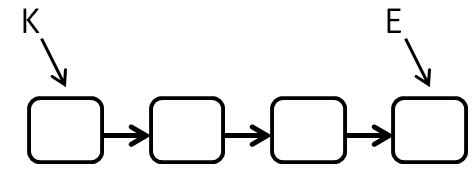
\includegraphics[width=6cm]{images/QueueListe}\\
	Anm: K muss auf den Listenanfang zeigen, da nur hier das Löschen in konstanter Zeit möglich ist.
\item \textit{ENQUEUE(x)}\\
	01 \tab \textbf{if} (E == \textit{NIL})\\
	02 \tab \tab E = x;\\
	03 \tab \textbf{else\\}
	04 \tab \tab  E.next = x;\\
	05 \tab \tab E = E.next;\\
	\ \\
	\textit{DEQUEUE()}\\
	01 \tab \textbf{if} (K == \textit{NIL})\\
	02 \tab \tab \textbf{error}(''Underflow!'');\\
	03 \tab \textbf{else}\\
	04 \tab \tab x = K;\\
	05 \tab \tab K = K.next;\\
	06 \tab \tab \textbf{return} x;
\end{itemize}

\item Löschen Sie in folgendem Rot-Schwarz-Baum das Element mit dem Schlüssel 17 und zeichenen Sie den Baum nach Ablauf der Operation. Sie können dabei die schwarzen Knoten durch einen doppelten Kreis kennzeichnen, die roten durch einen einfachen. (5P)\\

\begin{center}
\begin{tikzpicture}[level 1/.style={level distance = 1.2cm}, level 2/.style={sibling distance=50mm}, level 3/.style={sibling distance=30mm}, level 4/.style={sibling distance=12mm}, scale=1, level 5/.style={sibling distance=6mm}, scale=1]
   \node {}
    child {node [bvertex] {13} edge from parent[niceedge]
     child {node [rvertex] {8}
      child {node [bvertex]  {1}
      	child {node [nilvertex] {\nil}}
      	child {node [rvertex] {6}
	 child {node [nilvertex] {\nil}}
      	 child {node [nilvertex] {\nil}}
	}
      }
      child {node [bvertex]  {11}
      	child {node [nilvertex] {\nil}}
      	child {node [nilvertex] {\nil}}
      } 
    }
    child {node [rvertex] {17}
     child {node [bvertex] {15}
      child {node [nilvertex] {\nil}}
      child {node [nilvertex] {\nil}}
     }
     child {node [bvertex] {25}
      child {node [rvertex] {22}
       child {node [nilvertex] {\nil}}
       child {node [nilvertex] {\nil}}
      }
      child {node [rvertex] {27}
       child {node [nilvertex] {\nil}}
       child {node [nilvertex] {\nil}}
      }
     }
    }
   };
\end{tikzpicture}
\end{center}

\textbf{Lösung:} \\

Knoten 17 ist kein Blattknoten, kann also nicht direkt entfernt werden.
Er muss also zuerst mit einem Blattknoten getauscht werden. Dabei stehen zwei Kandidaten zur Auswahl:
Die 15 und die 22. Es ist offensichtlich einfacher, die 22 zu tauschen, denn rote Knoten sind unproblematisch.
Man tauscht also die 17 mit der 22 und entfernt die 17 anschließend. Dann ist man sofort fertig.\\
Für Gourmets: \textit{(die unbedingt die 15 tauschen wollen)}\\
Nach dem Tauschen und Entfernen des Knotens ist das linke NIL-Element (unter der 15) der Knoten x. Der Bruder ist also die 25, die selber schwarz ist und zwei rote Kinder hat.
Laut Vorlesungsfolien tritt also Fall 4 auf. Es muss rotiert werden (nach links um die 15) und umgefärbt. Damit ist die Reparatur abgeschlossen.

\end{enumerate}

\pagebreak
\section*{Aufgabe 6: Graphen (12 Punkte)}
\begin{enumerate}[(1)]
\item Ein Graph G = (V,E) sei durch die folgende Adjazenzfelddarstellung gegeben:\\
\ \\
V := \begin{tabular}{|c|c|c|c|c|c|}
\hline 
1 & 3 & 4 & 6 & 9 & 11 \\ 
\hline 
\end{tabular}  \\
\ \\
E := \begin{tabular}{|c|c|c|c|c|c|c|c|c|c|c|}
\hline 
2 & 3 & 4 & 2 & 5 & 2 & 3 & 6 & 1 & 6 & 5 \\ 
\hline 
\end{tabular}\\
\begin{enumerate}[(a)]
	\item Zeichnen Sie den Graphen. (2P)\\
	\textbf{Lösung:}\\
	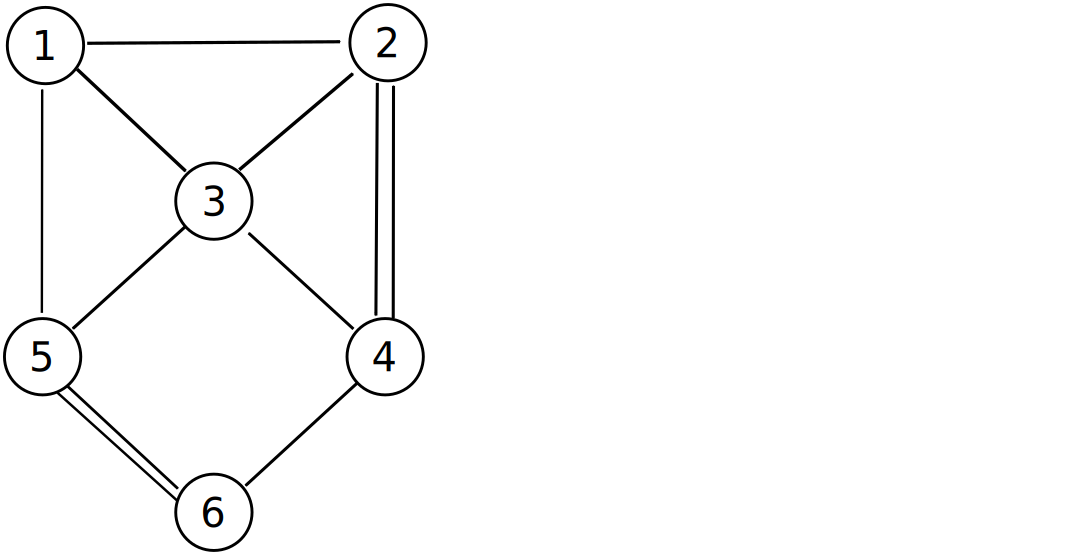
\includegraphics[width=5cm]{images/Graphdarstellungsaufgabe}
	\item Geben Sie den Graphen in Adjazenzlistendarstellung an. (1P)\\
	\textbf{Lösung:}\\
	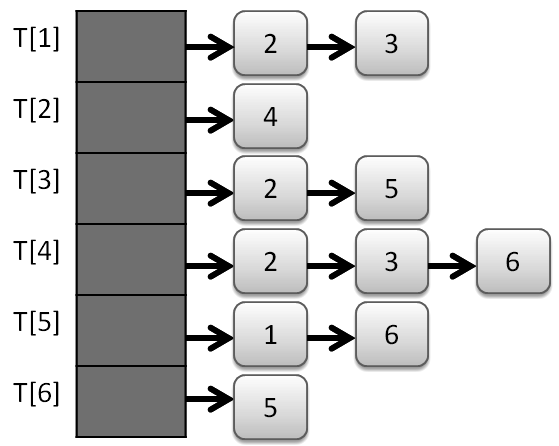
\includegraphics[width=6cm]{images/AdjazenzlisteSW}
	\item Welche dritte Möglichkeit zur Darstellung von Graphen wurde in der Vorlesung vorgestellt? Beschreiben Sie sie kurz und nennen Sie sowohl einen Vor- als auch einen Nachteil dieser Methode. (2P)\\
	\textbf{Lösung}\\
	Die dritte vorgestellte Möglichkeit ist die Adjazenzmatrixdarstellung. In einer $|V| \times |V|$-Matrix $A$ wird an der Stelle $A_{i,j}$ eine 1 gesetzt, wenn zwischen den Knoten i und j eine Kante existiert, andernfalls eine 0.\\
	Vorteile:
	\begin{itemize}
		\item Problem ''Existiert Kante von i nach j?'' in konstanter Zeit lösbar
		\item Einfaches Hinzufügen und Löschen von Kanten möglich
		\item manche Graphenoperationen direkt durch Matrixoperationen durchführbar (z.B. ''Existiert ein Pfad von A nach B?'' durch Potenzieren der Adjazenzmatrix)
	\end{itemize}
	Nachteile:
	\begin{itemize}
		\item verhältnismäßig hoher Speicherverbrauch bei dünnen Graphen
	\end{itemize}
\end{enumerate} 

\item Wenden Sie den Algorithmus von Prim auf dem folgenden Graphen an. Der Startknoten sei \textbf{a}. Markieren Sie die Kanten des resultierenden MSTs eindeutig (z.B. durch dicke Linien) und geben Sie die Reihenfolge der hinzugefügten Kanten an. (2P)
\begin{figure}[h]
\centering
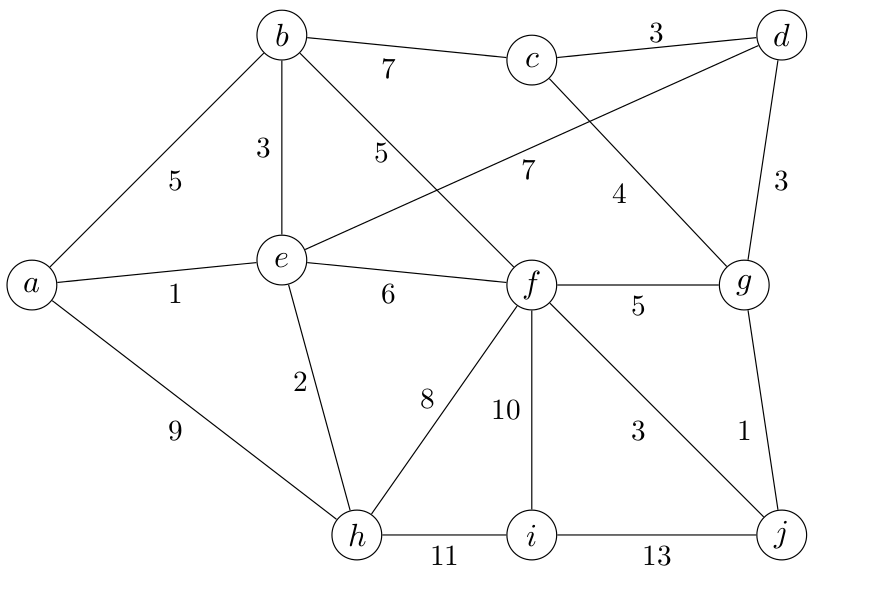
\includegraphics[width=0.66\textwidth]{mst_graph.png}
\end{figure}\\
\textbf{Lösung:}\\
\begin{figure}[h]
\centering
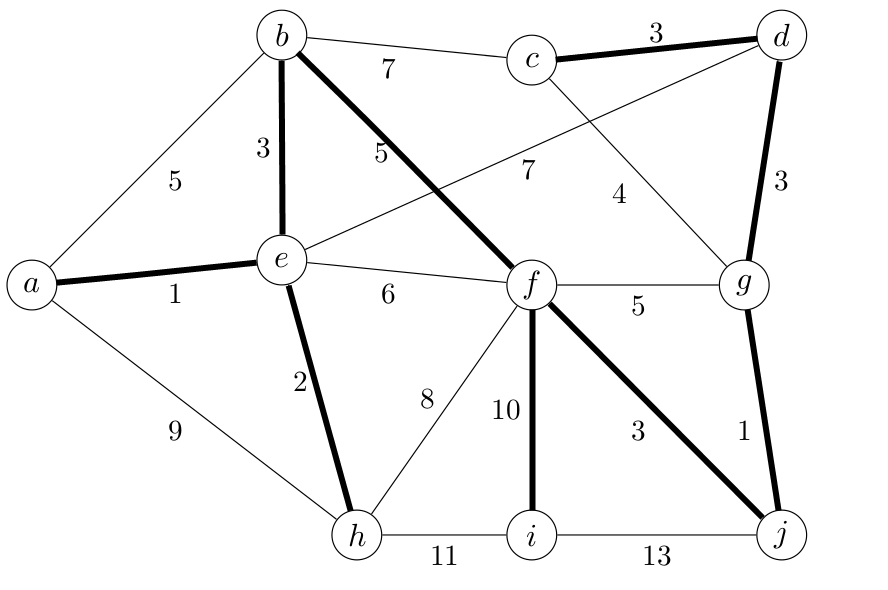
\includegraphics[width=0.66\textwidth]{images/mst_loes.png}
\end{figure}\\
Reihenfolge der Kanten: (a, e); (e, h);
\pagebreak
\item Gegeben sei folgender Graph:\\
\ \\
\begin{center}
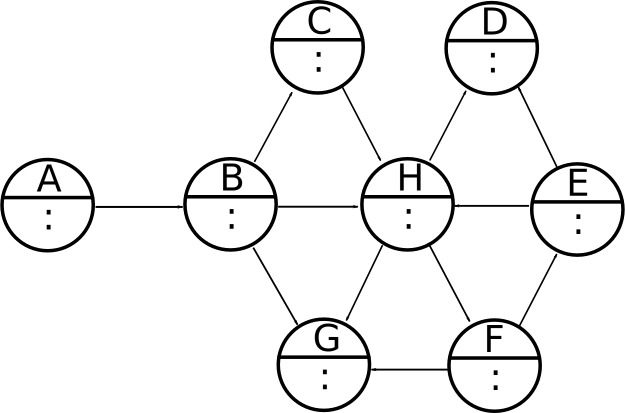
\includegraphics[width=0.75\linewidth]{images/tiefensuche_aufg}\\
\end{center}
Führen Sie auf diesem Graphen eine Tiefensuche aus und gehen Sie dabei wie folgt vor:
\begin{itemize}
	\item Beginnen Sie bei Knoten A.
	\item Betrachten Sie die ausgehenden Kanten eines Knotens bei der Suche jeweils im Uhrzeigersinn.
	\item Schreiben Sie die \textit{discovered}-Zeiten der Knoten links neben die Doppelpunkte, die \textit{finalized}-Zeiten jeweils rechts daneben.
	\item Klassifzieren Sie die Kanten. Kennzeichnen Sie dabei:
	\begin{itemize}
		\item jede \textit{Baumkante} durch eine dicke Linie
		\item jede \textit{Rückwärtskante} mit einem ''B''
		\item jede \textit{Vorwärtskante} mit einem ''F''
		\item jede \textit{Querkante} mit einem ''C''
	\end{itemize} 
\end{itemize}
(5P)
\end{enumerate}
\end{document}